
%% CLASS MANUAL FOUND IN http://blog.poormansmath.net/latex-class-for-lecture-notes/ %%
%% CLASS AUTHOR Stefano Maggiolo %%
\documentclass[english,course]{Notes}

\title{Network \& Operation Systems Essentials}
\subject{Computer Science}
\author{Joao Almeida-Domingues}
\email{2334590D@student.gla.ac.uk}
\speaker{Dr Nikos Ntarmos}
\date{24}{09}{2018}
\dateend{04}{12}{2019}
\place{University of Glasgow}

\graphicspath{{assets/}}

%%%%%%%%%%%% BIB CONFIG %%%%%%%%%%%%%%%
\usepackage[backend=biber, style=reading, citestyle=numeric]{biblatex} 
\usepackage{csquotes}
\newcommand\quo[1]{\begin{displayquote}\ita{\large{#1}}\end{displayquote}}
\bibliography{OOSE} %add bib file name

%%%%%%%%%%% LAYOUT  %%%%%%%%%%%%%%%

\renewcommand{\abstractname}{\vspace{3\baselineskip}} %hack to remove abstract
\usepackage{setspace}
\onehalfspacing

\lstset{
  basicstyle=\ttfamily,
  columns=fullflexible,
  frame=single,
  breaklines=true,
 }
%%%%%%%%%%%%%%%%%%%%%%%%%%%%%%%%

%%%%%%%%%%%%%% KEEP HERE (conflict when in class) %%%%%%%%%%%%%%%%%%%%

 %%%%%MATRICES
    
    \let\mat=\spalignmat
    \let\amat=\spalignaugmat
    \let\vec=\spalignvector
    
%%%%%% row ops
    \newcommand\ro[2]{\xrightarrow[#2]{#1}}
%%%%%%%%%%%%%%%%%%%%%%%%%%%%%%%%%%%%%%%%%%%%%%%%%%%%%

%%%%%%%%%%%%%  PACKAGES (NOT INCLUDED IN CLASS) %%%%%%%%%%%%%%
\usepackage[delims={[]}]{spalign}

%%%%%%%%%%%%%%%% ALGORITHM TEMPLATE %%%%%%%%%%%%%%%%%%%%

%\begin{algorithm}[H]
%\SetAlgoLined\KwData{this text}
%\KwResult{how to write algorithm with \LaTeX2e }initialization\;
%\While{not at end of this document}
%	{read current\;\eIf{understand}{go to next section\;current section becomes this one\;}{go back to the beginning of current section\;}}
%	\caption{How to write algorithms}
%\end{algorithm}

%%%%%%%%%%%%%%%%%%%%%%%%%%%%%%%%%%%%%%%%%%%%%%%%%%%%%

\begin{document}

%%%%%%%%%%%%%%  DISCLAIMER  %%%%%%%%%%%%%%%%%%%%%

\begin{abstract}
	\par{These lecture notes were collated by me from a mixture of sources , the two main sources being the lecture notes provided by the lecturer and the 
content presented in-lecture. All other referenced material (if used) can be found in the \ita{Bibliography} and \ita{References} sections.}
	\par{The primary goal of these notes is to function as a succinct but comprehensive revision aid, hence if you came by them via a search engine , please note 
that they're not intended to be a reflection of the quality of the materials referenced or the content lectured.}
	\par{Lastly, with regards to formatting, the pdf doc was typeset in \LaTeX , using a modified version of Stefano Maggiolo's \href{http://blog.poormansmath.net/
latex-class-for-lecture-notes/}{\underline{\textcolor{blue}{class}}}}
\end{abstract}
\newpage
\newpage

%%%%%%%%%%%%% LECTURES %%%%%%%%%%%%%%%%%%%%%%%

\section{Networks}

\subsection{Introduction - Networked Systems}

	\defn{Networked System}{a collection of autonomous computing devices that exchange data to perform some goal}

	\par{In this first part of the course we'll focus on 3 key aspects of these systems (1) how information is exchanged between the different devices involved ; (2) how we can build larger networks by linking devices ; (3) how systems communicate amongst themselves}

	\defn{Signal}{a function which conveys information}

	\defn{Communication Channel}{component of a a data transfer system responsible for carrying the signal}


	\defn{Information Entrophy}{how much useful information a message is \ita{expected} to contain}

	\par{\ita{Claude Shannon} the father of \ita{Information Theory} showed that the amount of information that can be coded into a message could be quantified, and is known as \ita{Information Enthropy}. Shannon stated that a data transfer system is composed of three parts: a source, a communication channel and a receiver. He identified the main problem within the system was to make sure that the information passed over the channel could be successuflly \ita{recreated} by the source.}

	\par{This encoding and decoding of messages can be done in several ways, some introduce more noise than others, but they all follow the same process of taking some form of physical signal (e.g. a wave) and converting it into some sort of simplied form of itself and then recreating it at the source end}

	\extra{Extra}{Information Enthropy Formal Definition}{
		\par{If we take $X$ as the set of messages $\{x_1 , \dots , x_n\}$ } 
		}

	\defn{Analogue Signal}{a smooth continuum of values}

	\defn{Digital Signal}{a discrete sequence of values}

	\par{The simplest analogue signal is when information is encoded directly using amplitude (e.g. AM radio), however of particular interest to us is the process of converting analogue signals to digital, which can be done for any analogue signal. (see Physical Layer) \rem{the the rate at
	which the signal must be sampled for accurate
	reconstruction is given by the sampling theorem}}

	\subsubsection{Switching}


	\defn{Coding}{the act of mapping information to symbols}

	\defn{Link}{the combination of a signal with a channel}

	\defn{Hosts}{receivers and sources}

	\defn{Network}{a collection of connected links}

	\par{Within a networked system, information flows via channels forming links which connect hosts. The devices connecting the links are called \ita{switches} or \ita{routers} depending on the type of network. This \ita{network switching} is responsible for determining how the information flows through the network and can be setup so that there are dedicated connections between hosts - \ita{circuit switching} - or by splitting the messages into smaller packets before transmission allowing several hosts to share the same channell - \ita{packet switching}}

	\defn{Circuit Switching}{a dedicated circuit between hosts}

	\defn{Packet Switching}{a shared link where messages are split into packets before transmission}

	\par{The main trade-off here is between capacity and availability. For example, traditional phone networks are circuit switched (the very first ones had actual humans switching the channels and connecting hosts) which means that the two hosts requested a channel and they had guaranteed capacity over that channel while the connection was active, but it also meant that if some other hosts needed to use any part of the same link then their connection would be refused.}
	\par{The internet on the other hand, is packet switched, by breaking the messages apart into smalled chunks hosts can share links the catch here being that though connectivity is guaranteed the capacity/speed is dependent on how many users are using the same channel.}



\subsection{Protocols}

	\par{The different building blocks of a network presented above allow for the transportation of information, but is is the use of protocols which provide the semantics. For a message to be decoded the parties involved must agree on some sort of well-defined syntax, so that noise can be separated from meaningul information, this is precisely the role of the various network protocols existing at all levels within a network.}

	\defn{PDU}{stands for protocol data unit, and is the basic unit	of information for any given protocol}

	\par{PDUs can be textual where rules of syntax and grammar are used to implement behaviour (e.g. HTTP), or binary where similar appropriate rules are used (e.g. TCP/IP). It is the role of PDUs to define what messages are legal to send, but is up to protocol semantics to define when to send them and what should be expected in response}

\subsubsection{Layers}

	\par{Communication systems are tipically organised into layers, which reduces complexity at each layer's level. Peers on the same layer, use that layer's protocol to communicate using services provided by the well-defined interfaces of the lower layers}

	\defn{OSI Model}{stands for \ita{Open Systems Interconnection Model} and is a conceptual model that characterises and standardises the communication functions of a telecommunication or computing system without regard to its underlying internal structure and technology. }

	\par{A design tool used widely to model layered communication channels is the \ita{OSI model}. It is merely a design tool, real implementations are more complex and usually the boundaries between layers are not so well defined.}

	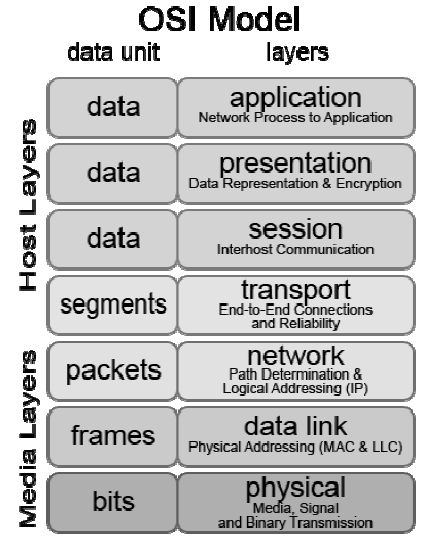
\includegraphics{osi.png}

\subsection{OSI - Physical Layer}

	\par{The physical layer is concernerd with the transmission of raw data bits. In order for this to be possbile, the information needs to be transformed and encoded and a decision on the best medium for the job (e.g. cables, fibre optic etc.) and their phyiscal properties needs to be taken.}

	\subsubsection{Transmission Channels - Enconding \& Modulation}

	\defn{Wired Data Trasmission}{ the signal is transmited over a cable and is \ita{directly} enconded onto the channel, by varying the voltage/light intensity}

	\defn{Wireless Data Transmssion}{ the signal is transmitted without the aid of an electrical conductor, most commonly using radio waves and some kind of modulation}

	\par{A signal can travel with or without the aid of an electrical condutor, if it is directly encoded into a cable, then one of several \ita{enconding schemes} can be used in order to change the signal into discrete pieces of data (e.g. bits).}

		\begin{itemize}
			\setlength\itemsep{0.5em}
			\mymarginpar{High $\approx [3,5]v$ , and Low $\approx [0,3)$}
			\mymarginpar{NRZ : Non-Return to Zero}
			\item\textbf{NRZ : }{1 -- High ; 0 -- Low}
			\item\textbf{NRZ Inverted : }{1 -- Change ; 0 -- Constant}
			\item\textbf{Manchester : }{1 -- High-Low ; 0 -- Low-High}
		\end{itemize}
		

		\todo{Insert image from anki card}

	\par{Alternatively one can encode information onto a channel by varying the properties of the carrier signal via a modulating signal, a process know as \ita{modulation} which allows the same channel to be shared by different signals}

		\todo{Insert image from anki card}

	\subsubsection{Bandwith, Capacity \& Noise}

	\defn{Bandwith}{ determines the frequency range it can transport}

	\defn{Sampling Theorem}{ states that to accurately digitise an analogue signal, $2H$ samples per second are needed, where $H$ is the bandwith in Hz}

	\defn{Signal-to-Noise Ratio}{ the ration between signal power and noise floor, typically quoten in dB $= 10\log(\frac{S}{N})$}

	\par{The bandwidth of a channel is determined by physicial limitations of the channel, and given the existence of noise in the real worl, the \ita{Signal-to-Noise} ratio and the bandwidth represent the fundamental limits for the rate at which information can be transmitted}

	\rem{The maximum transmission rate of a channel grows lograithmically to the SNR}

	\extra{Extra}{Theoretical Maximum Transmission Rate}{

		$$ R_{max} = 2H\log_{2}V $$

		where:
		\begin{itemize}
			\item[]$R_{max} =$ max trasmission rate in bits/s
			\item[]$H =$ bandwith in Hz
			\item[]$V =$ \# of discrete values per symbol
		\end{itemize}
	}

	\extra{Extra}{Shannon's Theorem}{
		$$ R_{max} = H\log_{2}(1 + SNR) $$

	}

	


	
	\subsubsection{Summary}

		\begin{itemize}
			\item\textbf{PDU : } bits
			\item\textbf{Function : } transmit a sequence of bits over an analogue channel
		\end{itemize} 

\subsection{OSI - Physical Layer}

	\par{The physical layer is concernerd with the transmission of raw data bits. In order for this to be possbile, the information needs to be transformed and encoded and a decision on the best medium for the job (e.g. cables, fibre optic etc.) and their phyiscal properties needs to be taken.}

	\subsubsection{Transmission Channels - Enconding \& Modulation}

	\defn{Wired Data Trasmission}{ the signal is transmited over a cable and is \ita{directly} enconded onto the channel, by varying the voltage/light intensity}

	\defn{Wireless Data Transmssion}{ the signal is transmitted without the aid of an electrical conductor, most commonly using radio waves and some kind of modulation}

	\par{A signal can travel with or without the aid of an electrical condutor, if it is directly encoded into a cable, then one of several \ita{enconding schemes} can be used in order to change the signal into discrete pieces of data (e.g. bits).}

		\begin{itemize}
			\setlength\itemsep{0.5em}
			\mymarginpar{High $\approx [3,5]v$ , and Low $\approx [0,3)$}
			\mymarginpar{NRZ : Non-Return to Zero}
			\item\textbf{NRZ : }{1 -- High ; 0 -- Low}
			\item\textbf{NRZ Inverted : }{1 -- Change ; 0 -- Constant}
			\item\textbf{Manchester : }{1 -- High-Low ; 0 -- Low-High}
		\end{itemize}
		

		\todo{Insert image from anki card}

	\par{Alternatively one can encode information onto a channel by varying the properties of the carrier signal via a modulating signal, a process know as \ita{modulation} which allows the same channel to be shared by different signals}

		\todo{Insert image from anki card}

	\subsubsection{Bandwith, Capacity \& Noise}

	\defn{Bandwith}{ determines the frequency range it can transport}

	\defn{Sampling Theorem}{ states that to accurately digitise an analogue signal, $2H$ samples per second are needed, where $H$ is the bandwith in Hz}

	\defn{Signal-to-Noise Ratio}{ the ration between signal power and noise floor, typically quoten in dB $= 10\log(\frac{S}{N})$}

	\par{The bandwidth of a channel is determined by physicial limitations of the channel, and given the existence of noise in the real worl, the \ita{Signal-to-Noise} ratio and the bandwidth represent the fundamental limits for the rate at which information can be transmitted}

	\rem{The maximum transmission rate of a channel grows lograithmically to the SNR}

	\extra{Extra}{Theoretical Maximum Transmission Rate}{

		$$ R_{max} = 2H\log_{2}V $$

		where:
		\begin{itemize}
			\item[]$R_{max} =$ max trasmission rate in bits/s
			\item[]$H =$ bandwith in Hz
			\item[]$V =$ \# of discrete values per symbol
		\end{itemize}
	}

	\extra{Extra}{Shannon's Theorem}{
		$$ R_{max} = H\log_{2}(1 + SNR) $$

	}

	
	\subsubsection{Summary}

		\begin{itemize}
			\item\textbf{PDU : } bits
			\item\textbf{Function : } transmit a sequence of bits over an analogue channel
			\item Information can be encoded directly into the channel or the signal can be modulated
			\item Physicial limitations cap the transfer rate
		\end{itemize} 
\subsection{OSI - Data Link Layer}

	\par{The main purpose of the data link layer is to arbitrate access to the physical layer and turn the raw bit stream of data into a structured communications channel with the goal of transferring data between nodes attached to the same physical cable. There are several services provided by the DDL, the main ones being: \ita{Media Access Control (MAC addressing) , Error detection and/or correction, Framing}}


	\subsubsection{Framing}

		\par{Frames are essentially fenced packets, which signal to the next layer the significant part of the data , i.e the \ita{payload} and often whether that data was corrupted via some sort of error code or \ita{checksum}. The DLL add the final tail and header to the payload and is therefore responsible for the last bit of data \ita{encapsulation}}

		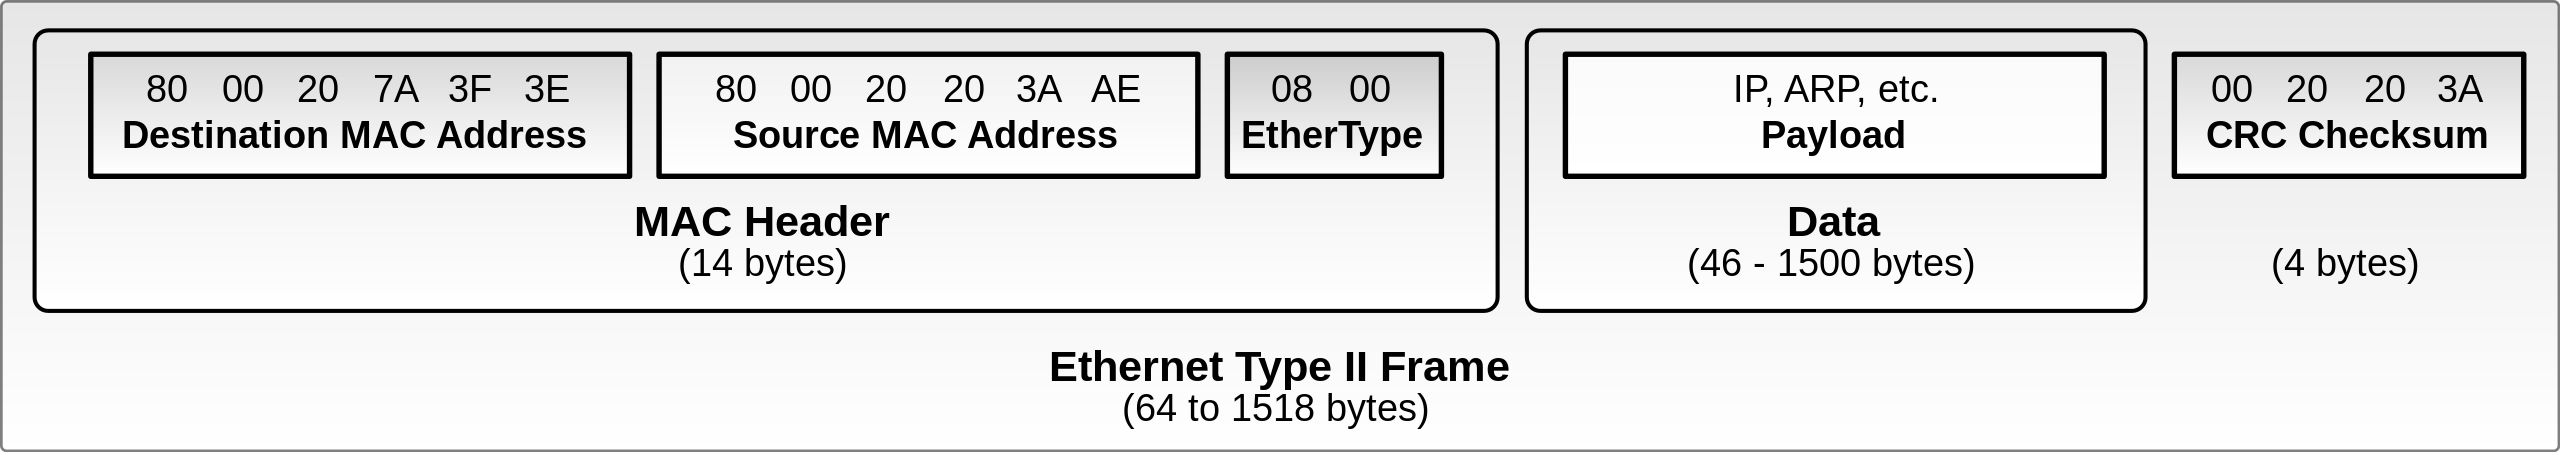
\includegraphics[width=0.7\textwidth]{frame}


	\subsubsection{Error Detection \& Correction}

		\par{Though rare in wired systems, it is quite common for noise to cause bit errors in the data being transmitted. If the DLL implements error detection then it must add a \ita{error detection code} as an header of the frame, the simplest one being the \ita{parity code}. When the receiver gets the packet it uses the same function/rule to recalculate the code, if it doesn't match the frame is either discarded or corrected}

		\defn{Parity Code}{an error detection code which is able to detect single bit errors. It works by adding all the bits, and checking the parity of their sum}

		\defn{Checksum}{works similarly to the parity code, but is able to handle some multiple bit errors by using a 16-bit one's complement checksum}

		\defn{Cyclic Redundancy Code}{a more advanced algorithm, commonly used in the DDL which can check if the bits are out of order. It relies on the remainder of a polynomial division of the data being sent}


	\subsubsection{MAC}

		\par{MAC is needed to determine which machine gets access to the channel when multiple hosts try to access it simultaneously. Because if that happens then the signals are said to \ita{collide} and will overlap, resulting in an unreadable/garbage message.}

		\defn{Contention-Based MAC}{a system is contention-based if multiple hosts share a channel in a way that can lead to collisions}

		\par{CB MAC deals with collision in one of two ways:}

			\begin{enumerate}
				\item \textbf{ALOHA} is the simplest protocol developed at the University of Hawaii in 1970. It tries to transmit whenever data is available, and if a collision occurs the frames are destroyed and the node will wait for a random amount of time before retransmitting, repeating until successful.

				\item \textbf{CSMA} listens to the channel before sending, if it hears no traffic then it starts transmitting. Note however, that if the message takes time to reach the node , i.e. if there's a high \ita{propagation delay} then there is an increased probability of a collision occurring mid-transit, an improved algorithm is \textbf{CSMA/CD} where the sending node keeps listening even during sending, if a collision occurs then both stations cease transmission immediately. This is an improvement because even though the frames are still corrupted, it saves time and bandwidth by reducing the time the channel is blocked due to collision.
				\mymarginpar{The back-of interval between retransmissions is also random, but should increase with the number of collisions to reduce congestion}
			\end{enumerate}

	




	\subsubsection{Summary}
		\begin{itemize}
			\item\textbf{PDU : } series of bits - \ita{frame}
			\item\textbf{Function : } Physical addressing , Framing, Error Detection
			\item Last encapsulation of data step ; adds an error detection code and some other meta data for framing in the trail of the packet
			\item Simpler error detection codes rely on summing up the bits of data and either checking their parity or sum
			\item Contention-Based MAC handle collisions by listening to the channel before sending the data and/or during
		\end{itemize}

\subsection{OSI - Network Layer}

	\defn{End-to-End Principle}{is a network design principle whereby application-specific features reside in the end nodes, rather than being distributed across the network}

	\par{The Network layer is responsible for end-to-end delivery of data and is therefore the first end-to-end layer in the OSI. This is important because networks can be of enourmous sizes, and since implementing a function always has a cost, if that function is implemented across the whole of the network that cost quickly multiplies. If instead the system is concerned with achieving reliability of communication above a certain threshold, it is more efficient to implement processes for checking for correctness and completeness at the end hosts rather than at the intermediary nodes, since end-to-end reliability is not perfectly aligned with the reliability of intermediary processes}

	\defn{Internet}{set of interconnect networks}

	\defn{Autonomous System}{a network within a larger network which is administered separately by a single organisation who is responsible for making independent policy and technology choices}

	\par{The basic components of an internet are:}

	\begin{enumerate}
		\item The existence of a common end-to-end protocol, which provides a single seamless service to the transport layer
		\item A set of intermediate gateway devices, i.e routers, which implement the protocol and hide differences in link layer technologies by performing the usual services provide by that layer
	\end{enumerate}

	\subsection{Network Layer - Internet Protocol}

	\par{The IP provides an abstraction layer, including a \ita{simple, best effort, connectionless} packet delivery service. Which means, that it does not guarantee correctness or delivery, but it allows for addressing, routing, fragmentation and reassembly of packets.}
	\par{The IP service model does not require a connection to be setup first, instead it just sends the available packets and anything which cannot be delivered is discarded. This means that it favours simplicity over assurance and correctness, leaving that for the layers above.}

			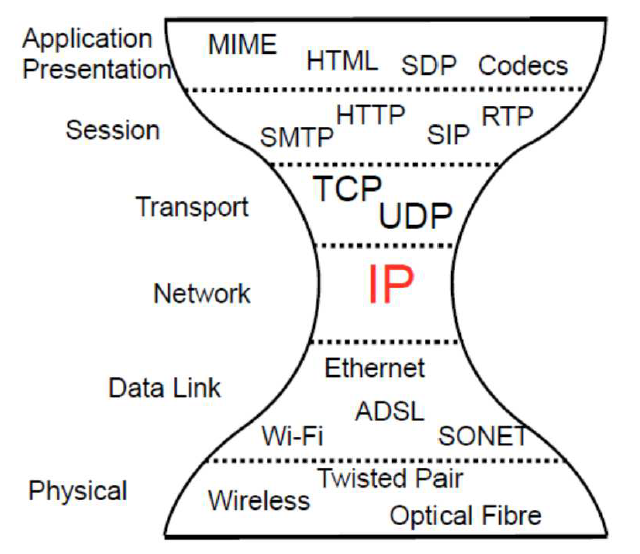
\includegraphics[height=0.3\textheight]{protocols.png}

			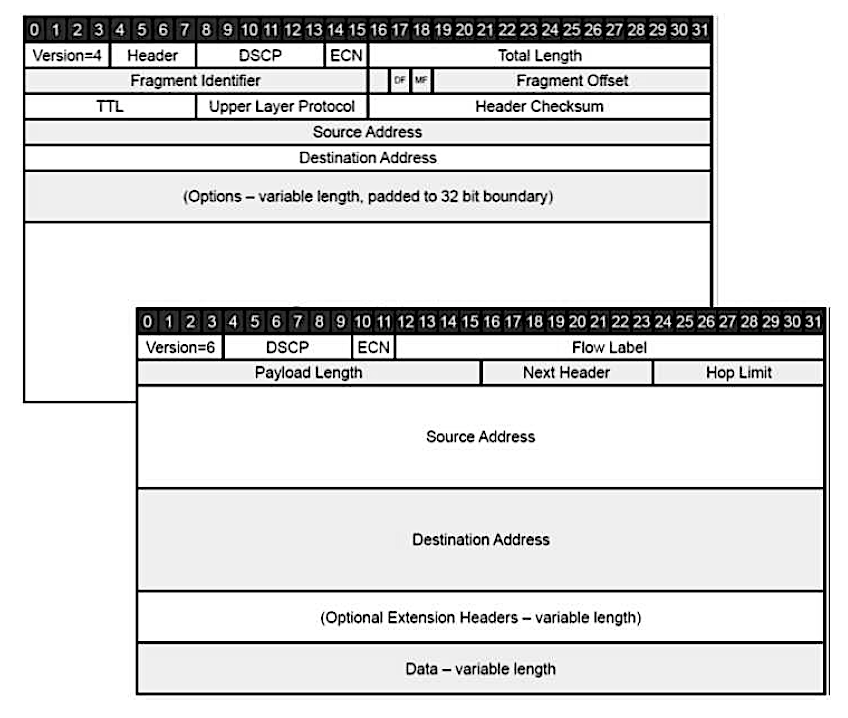
\includegraphics[width=0.7\textwidth , height=0.3\textheight]{ip_dataframe.png}

	
	\subsubsection{Addressing}

		\par{IPv4 addresses are 32 bits ($4\times8$), while IPv6 are 128 bits ($16\times8$), one part of the address identifies the network while the other identifies the host (which part is which may vary across different networks). Each network interface must have an unique address, however virtual IP addresses are sometimes used to give the illusion of privacy}

	\rem{IPv4 addresses are deemed insufficient for the near future, so IPv6 was created. It has been slowly deployed since 2000 given the costs of replacing hardware and updating current software}

		\defn{netmask}{describes the number of bits reserved for the network part of the address}
	
		\defn{network address}{the host part of the address is set to 0}

		\defn{broadcast address}{the host bits are set to 1}

			$$
			\begin{array}{l}
			\text { IP address: } 130.209 .241 .197 \Rightarrow  \ 11010001 \ 11110001 \ 11000101 \\ 
			\text { Netmask: } 255.255 .240 .0 \Rightarrow11111111 \ 1111111 \ 11110000 \ 00000000 \\ 
			\text { Network: }130.209 .240 .0 / 20 \Rightarrow 10000010 \ 11010001 \ 11110000 \ 00000000 \\ 
			\text { Broadcast: } 130.209 .255 .255 \Rightarrow 10000010 \ 11010001 \ 11111111 \ 11111111
			\end{array}
			$$

		\rem{a host with several network interfaces will have one IP address per interface (e.g Ethernet and WiFi interfaces in a single machine)}

	\subsubsection{Fragmentation}

		\defn{Fragmentation}{process which breaks packets into smaller fragments so that a layer with a smaller maximum transmission unit can receive them}

		\par{The link layer has a MTU, hence before sending the packets to it, the IP breaks the packets apart into smaller frames. The process is reversed when receiving, and this can be achieved by including metadata with each frame - the \ita{fragment identifier} , the \ita{DF, MF flags} and the \ita{fragment offset}. The DF flag is set if the packet is not to be fragmented, the MF flag lets the node know that it should expect more fragments part of the same packet.}

		\rem{Note that both the last fragment of a packet as well as an unfragmented packet have MF set to true. These two cases are differentiated by setting the offset to a non-zero value in the first case}

		\subsubsection{Loop Protection}

		\par{In order to ward against loops, packets include a value which sets the maximum number of hops allowed in the network. With each hop this value decreases and if 0 is reached the packet is discarded \mymarginpar{IPv4 - TTL ; IPv6 - Hop Limit}}

		\subsubsection{Transport Layer Protocol Identifier}

		\par{\mymarginpar{IPv4 - Upper Layer Protocol ; IPv6 - Next Header}The TLPI is responsible for identifying the protocol used by the Transport layer above, in order to pass the data to the correct one.}


\section{OS - Intro}

\defn{Operating System}{a program which acts as an intermediary between the user and the hardware}

\par{The OS is the software which allows the user and higher level applications to communicate with the metal. It serves 3 main purposes:}

\begin{itemize}
	\item Usability
	\item Program Execution Scheduling and Control
	\item Efficiency Allocation of Resources
\end{itemize}

\subsection{Core Components}

	\defn{Kernel}{the program running at all times which is responsible for providing and API for the interaction between hardware and higher level programs; performing such tasks as reading and writing data to memory and determining how data received from and sent by \ita{I/O} devices is interpreted.}

	\defn{System Programs}{are programs which despite being associated with the OS do not form part of the kernel, they provide a platform for apps}

	\defn{Application Programs}{are programs which do not interact with the OS directly}

	\defn{BIOS}{the \ita{Basic Input Output System} is a special piece of software which comes preinstaled in the system's board ROM and is responsible for checking that the hardware is operation and loading the OS}

\subsection{Computer System Organization}

	\defn{Computer System}{can be defined as the interaction between four main components: \ita{Hardware, OS, Application Programs, Users}}

	\par{A modern computer system consists of 1+ CPUs and a number of device controllers which interact via a common bus that provides access between components and shared memory. It is the job of the device controller to transfer data between the devices and the local buffer storage which it maintains along with a set of special-purpose registers.}
	\par{The CPU and the device controllers can execute in parallel, competing for memory cycles. The three key aspects of the computer-system - Interrupts, Storage Structure, I/O Structure - are deigned in such a way so as to allow for memory to be used as efficiently as possible }

	\begin{figure}[H]
		\begin{center}
		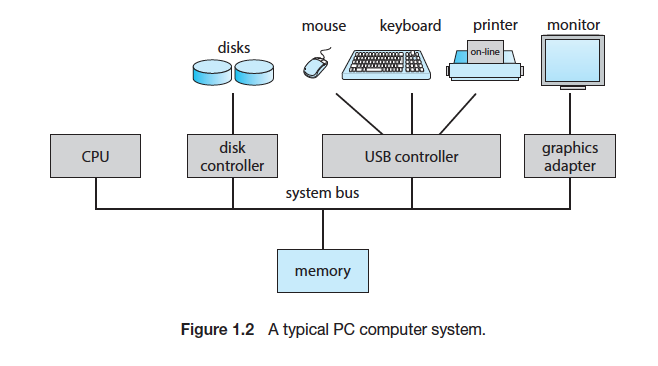
\includegraphics[width=\textwidth]{system}
		\end{center}
	\end{figure}


	\subsubsection{CPU Interrupts}

		\par{A typical operation of a program performing I/O:}

			\begin{enumerate}
				\item Device driver loads the registers in the controller
				\item Controller inspects data in order to know what action to execute
				\item Controller transfers data to local buffer
				\item Controller informs driver that operation has finished
				\item Driver gives back control to OS
			\end{enumerate}

		\par{The controller accomplishes 4 via an \ita{interrupt}. When hardware triggers an interrupt, the CPU stops the execution of all programs and it transfers execution to a fixed location which will usually contain the starting address for the interrupted service so that execution can restart when the interrupt routine finishes.}
		\par{Different architectures have different interrupt mechanisms, but they all share several essential functions, such as the transfer of control to the appropriate service routine. In order for this transfer to occur quickly a table of pointers to different interrupt routines - \ita{interrupt vector} - is kept in low memory and is used instead of an extra routine whose sole purpose would be to inspect the interrupt information. In this way the routine is called indirectly via the table.\mymarginpar{For implementation details see 1.2.1.2}}

		\begin{figure}[H]
		\begin{center}
		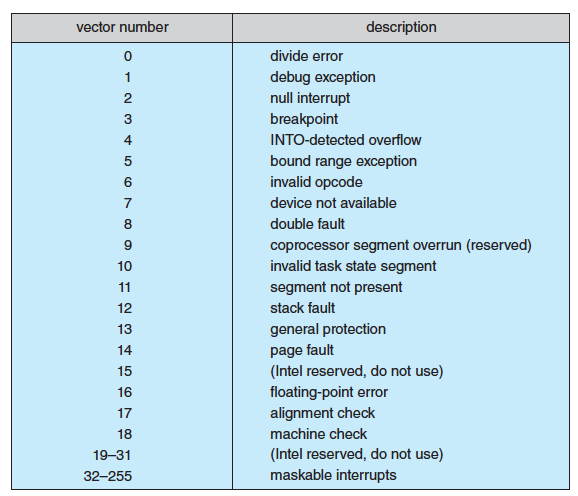
\includegraphics[width=\textwidth]{eventVector}
		\end{center}
	\end{figure}


	\subsection{Storage Structure}

	\par{When looking at a storage system one can pick out three main characteristics of importance, whose importance differs depending on their function and at which level of the system they are to be implemented, and which compete against each other. These are: \ita{Speed, Cost, Persistence/Volatility}}
	\par{Devices which need to process information immediately like the registers in the CPU are more costly,have a lower storage capacity and are in general volatile. In contrast, long-terms storage devices like the hard disk, or a flash drive are fairly inexpensive but their read/write speeds are significantly slower.}

	\begin{figure}[H]
		\begin{center}
		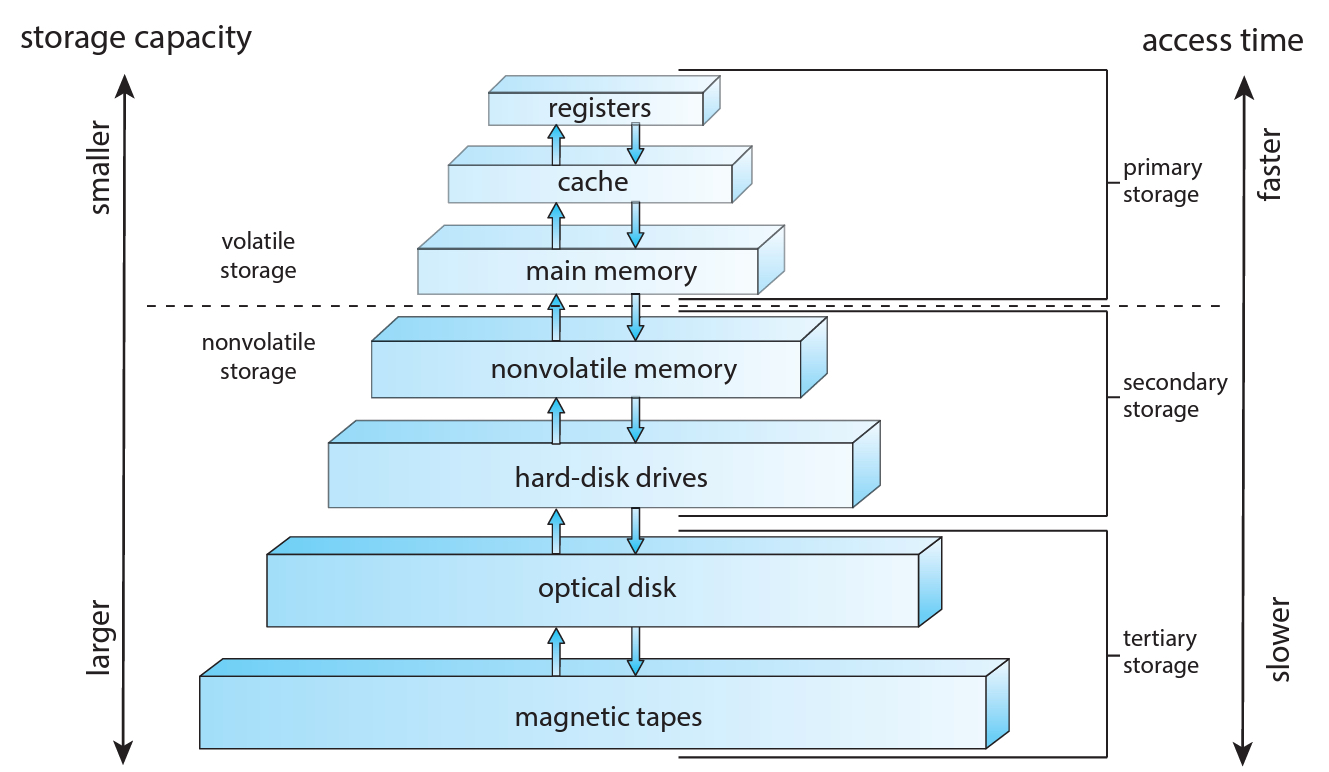
\includegraphics[width=\textwidth]{mem_hierarchy.jpg}
		\end{center}
	\end{figure}

	\defn{Caching}{the copy of information into faster storage systems}

	\subsection{I/O Structure}

	\par{A large chunk of OS code is dedicated to I/O management. Given the large amounts of data being moved by some I/O devices, the interrupt-driven cycle can produce high overhead instead direct memory access is used.}

	\defn{Direct Memory Access}{a resource-conserving and performance-improving operation for device controllers which allows devices to transfer large amounts of data directly to and from main memory, effectively bypassing the CPU and using instead a single purpose processor - \ita{DMAC}.}

\section{Computer-System Architecture}

	\par{The organization of a system can be categorized according to the number of general-purpose processors used.}

	\defn{Core}{the component that executes instructions and registers for storing data locally}

	\defn{CPU}{The hardware that executes instructions}

	\defn{Processor}{A physical chip that contains one or more CPUs}

	\subsubsection{Single-Processor}

	\par{The SP architecture uses a single CPU with a single processing core along with other device-specific processors which can only run a limited set of instructions.}

	\rem{This type of architecture is no longer present in modern computers}

	\subsection{Multiprocessor}

		\defn{Multicore}{a single CPU with more than one core who usually share some low-level memory}

		\defn{Throughput}{the amount of information which passes through the system}

		\par{Modern computers have 2+ processors each with a single core CPU. The processors share the computer bus, and may also share the clock, memory, and peripheral devices.The main advantage of this type of architecture is increased throughput, i.e. the higher number of processors allow for more data to be processed in less time}

		\rem{Increasing the number of processors by $N$ does not imply a $N$-fold increase in speed, since some of the processing power will be lost as overhead to tasks which make sure that the processors behave correctly when working together and sharing resources}

		\par{There are two main types of multiprocessor systems - \ita{Symmetric} and \ita{Asymmetric}, the former being the most common. They differ in the way tasks are split amongst different processors}

		\subsubsection{Symmetric}

			\par{In SMP each CPU processor performs all tasks, each CPU containing its own set of registers and private cache but all processors share access to the main memory. This has the advantage that many processes can run simultaneously\mymarginpar{$N$ processes can be running in a system with $N$ CPUs}. The downside of this type of system is that inefficiencies can occur by overloading one CPU while the other sits idle.}


		\subsubsection{Asymmetric}

			\par{Was the only way to handle multiprocessor systems before the invention of SMP. It is characterized by the fact that CPUs are not treated equally, i.e different CPUs prioritize certain tasks , like say I/O while others are reserved for system operations.}

	\subsection{Clustered}

		\par{The rationale behind clustered systems is similar to that of the multiprocessor systems, but we expand vertically, i.e instead of looking at multiple CPUs within a single computer, we use several computers within the same network.}
		\par{Clustered systems are very common nowadays and advancements in speed and computing power are linked to their pairing with SANs which are essentially local, dedicated data-storage networks. By having multiple machines connected to the same SAN if one machine goes offline another can quickly pick up the slack.}

		\defn{SAN}{describes a combination of hardware and software which essentially work together to form a dedicated storage area network}

		\defn{hot-standby mode}{one system runs parallel to another, in case the primary fails the backup quickly takes over}

		\defn{Asymmetric Clustering}{one machine in hot-standby mode}

		\defn{Symmetric Clustering}{multiple nodes running applications and monitoring each other}

\subsection{Process Management}

	\defn{Process}{a program in execution}

	\defn{Single-Thread}{single program counter which specifies the location of the next instruction to execute}

	\defn{Multi-Thread}{one program counter per thread}

	\par{In order to manage processes the system needs to be able to:}

		\begin{itemize}
			\item[]{Create and delete user and system processes}
			\item[]{Suspend and resume processes}
			\item[]{Provide mechanisms for process synchronization, communication and deadlock handling}
		\end{itemize}

\subsection{Memory Management}
	
	\par{Memory management is responsible for determining what is in memory, this includes:}

		\begin{itemize}
			\item[]{Tracking which parts of memory are in use and by whom}
			\item[]{Deciding which processes and data to move into and out of memory}
			\item[]{Allocate memory space as required}
		\end{itemize}

\subsection{Storage Management}

	\par{Storage management concerns itself with the management of the file-system, in particular how the OS handles free space and how that free space is split into files and directories with appropriate access permissions so that the user can easily access them.}




\section{System Calls}

	\defn{System Call}{the software, typically written in a high-level language (e.g C), which sits between the hardware and the applications}

	\defn{User mode}{restricted level where most programs run without direct access to memory or hardware}

	\defn{Kernel mode}{unrestricted program execution}

	\par{Programs running on user mode are provided an API by the OS which provides the application which mediated access to the hardware. A classical example is a basic task like writing to and reading from a file.}

	\subsection{Parameter Passing}

		\par{In order to pass parameters to the system call we can:}

		\begin{itemize}
			\item[] use registers
			\item[] stored them in memory and address of the block passed in register
			\item[] push onto the stack by the program and pop by OS
		\end{itemize}

	!! INSERT EXAMPLE OF SYSTEM CALLS TABLE !!

\subsection{Program Execution}

	\par{As we've seen above the difference between a program and process is that a process is a program being executed. Note than that one program can spawn several processes, i.e for the same file on disk (the written code) multiple requests to resources might happen (e.g multiple tabs on a browser)}

	\subsubsection{Process States}

	\defn{Ready Queue}{an array of active processes waiting to be run}

		\par{Once execution of a program starts a request to the OS is made and the process is added to the \ita{ready queue}. It will then be transitioned into the running state, it can then exit and terminate or can be put into waiting state and back into the ready queue until resources are available for it to finish execution.}

	!! INSERT DIAGRAM !!

	\defn{PCB}{is a data structure used by the OS to store all the information associated with a process}

		\par{For every process the OS keeps a PCB containing all information associated with it, such as state, numbers, counter etc.}

\subsection{Process Creation}

\defn{Process Tree}{}

\defn{Boot Loader}{is the program stored in the ROM responsible for loading data and programs into RAM}

\defn{Zombie Process}{}

\defn{Orphan Process}{}

	\par{Processes are spawned by other processes, creating what is know as a \ita{process tree}. When a machine starts there is a single process , the \ita{boot loader} which is responsible for loading the OS into the main memory, this is usually done in multiple stages where simpler programs load increasingly more complex ones, a process know as \ita{chain loading}.}
	\par{The system calls responsible for the creation of processes are:}

		\begin{itemize}
			\item[] \texttt{fork(2)} - takes a process and creates a copy of it
			\item[] \texttt{exec(3)} - family of functions which takes one of the processes and replaces its code with another program's code
			\item[] \texttt{wait(2)} - stops the running process and waits for one of its children to terminate
		\end{itemize}

	\par{By default parent and children processes run concurrently, and the parent waits for the children to terminate. There are multiple level of resource sharing, between sharing all to none.}

	\rem{It could happen that a parent process may fail to \ita{reap} its children state after execution, in which case a \ita{zombie} process is created, which keeps using resources in the background. If the opposite happens, i.e if the parent finishes first then the child process becomes \ita{orphan}}

	!! INSERT TREE !!


\section{Inter-Process Communication}

	\par{Processes can be independent running in isolation or cooperative sharing data. Cooperating processes can be affected by other processes, which can lead to a chain failure. However, cooperating processes can often be more efficient, since they share information, are more modular and more convenient to run.}

	\subsection{Communication Models}

		\par{It follows that if two processes are cooperating then they need to be able to communicate with each other. There are two possible modes of communication, \ita{message passing} and \ita{shared memory}. In the former processes communicate by sending calls to each other via a message queue in the latter a space of shared memory is allocated where  both processes can read and write.}
		\par{Both processes are often implemented within the same system. The shared memory model is particularly useful when large amounts of data need to be shared; it is also faster since it only uses system calls to establish the region in memory. The message passing model on the other hand is easier to implement in distributed systems, hence it is usually applied when small amounts of data need to be shared.}


	\subsubsection{Message Passing}

		\par{A message passing model has to provide at least two operations \texttt{send} , \texttt{receive}. There are however several factors to consider when implementing these:}

		\begin{itemize}
			\item Directly : If the communication is implemented \ita{directly}, then processes much name each other, if both the receiver and sender are named then the communication is said to be \ita{symmetric}. On the other hand, if only the recipient is explicitly named then one calls it \ita{asymmetric}. 
			\item Indirectly : If the communication is implemented \ita{indirectly} the messages are sent and received via \ita{mailboxes}. Unlike before, links are not necessarily $1-1$ since many processes can share a mailbox. Once a mailbox is created by an initial process, other processes access to the mailbox can be mediated via system calls.
			\item Synchronization : if when performing a \texttt{send, receive} the actor is blocked, then we say that the process is \ita{synchronous}, if the opposite is true then it is \ita{asynchronous}
			\item Buffering : The size of the queue can be either 0, in which case sender must wait for receiver; may be bounded by $n$, in which case the sender must wait if queue is full , or may be unbounded where the sender can keep adding to the queue without restrictions.

	\subsubsection{Shared Memory}


\section{Process Scheduling}

	\defn{I/O Bound}{a process which spends most of its time doing I/O instead of computations}

	\defn{CPU Bound}{a process which spends most of its time doing computations}

	\defn{Multiprogramming}{when theres a process running at all times}

	\defn{Time Sharing}{switch among several different processes quickly enough so as to give the impression of parallel execution}

	\defn{Long-Term Scheduler}{is responsible for maintaining a healthy balance between IO and CPU bound processes in memory}

	\defn{Medium-Term Scheduler}{swaps processes from active to passive and vice-versa}

	\defn{Short-Term Scheduler}{selects which process to execute next}

	\par{Even with multiple cores, if there are more processes then cores then some processes will need to wait before they're able to run. Hence, there is the need for some sort of scheduling of processes. The main goal of the scheduler is to maximize CPU utilization at all times, in order to achieve this there exist several types of schedulers and several queues need to be maintained in order to keep track of each process state.}

	\begin{figure}[H]
		\begin{center}
		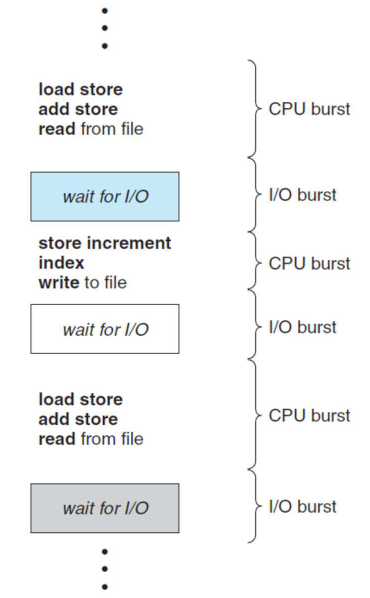
\includegraphics[width=0.75\textwidth , height=0.25\textwidth]{processLife}
		\end{center}
	\end{figure}

	\par{The \ita{job scheduler} concerns itself with loading programs into memory, the \ita{medium-term} one performs possibly necessary swaps between active/holding states and the \ita{CPU scheduler} decides which process to execute next. These 3 schedulers can move processes among the various queues : all processes exist first in the \ita{job queue}, once they are in RAM and ready to execute they are put into the \ita{ready queue}, if the process is waiting for a particular device then it is put into that device's queue.} 

	\begin{figure}[H]
		\begin{center}
		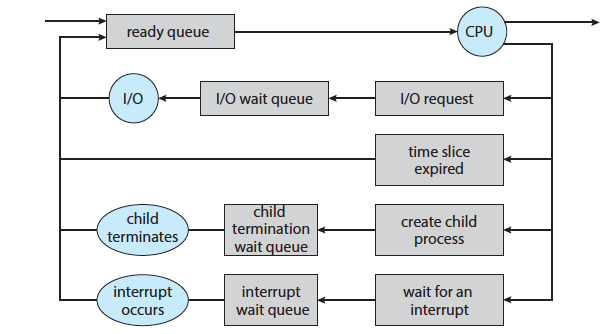
\includegraphics[width=\textwidth]{sched}
		\end{center}
	\end{figure}

	\subsection{CPU Scheduler}

		\defn{Non-Preemptive Scheduling}{let the process run its course without interruption}

		\defn{Preemptive Scheduling}{the process decides when the process should yield the CPU}

		\par{As discussed a process may switch several times between one of the queues and the CPU, though CPU bound processes will spend more time executing it is unlikely that the scheduler will grant long chunks of uninterrupted time to these processes. Instead, processes in the core are constantly interrupted and switched.}

		\rem{It is common for the CPU scheduler to execute much more frequently than once every 100ms}

		\par{When to decide when to schedule a process to run in the core may take place at any of 4 stages of a life of a process:}

			\begin{itemize}
				\item[] Running $\to$ Waiting (e.g I/O request)
				\item[] Running $\to$ Ready (e.g interrupt)
				\item[] Waiting $\to$ Ready (e.g I/O terminates)
				\item[] Termination 
			\end{itemize}

	\subsection{Dispatcher}

		\defn{Dispatch Latency}{is the time it takes the dispatcher to switch processes}

		\par{It is the job of the dispatcher to give control of the CPU to the process selected by the scheduler. In order to do this the scheduler must be able to \ita{switch context}, \ita{switch to user mode} and \ita{jump back to the proper instruction in the user program to resume execution}}

		\rem{Given that the dispatcher is called every time a process is swapped and the time it takes to do so is pure overhead, it is important that it be as fast possible. }

	\subsection{Scheduling Criteria}

		\par{The best algorithm for a particular process may not be the best for another set of processes. It is important that one is aware of this fact when choosing an algorithm. In order to compare them, the following criteria can be used:}

			\begin{itemize}
				\item[]CPU Utilization : maximize , in practice somewhere between $40\%-90\%$
				\item[]Throughput : maximize , for any given time unit, one aims to complete as many processes as possible 
				\item[]Waiting Time : minimize , waiting time is wasted time
				\item[]Turnaround Time : minimize , the aim is faster total completion times 
				\item[]Response Time : minimize , in an interactive system this criteria can be better than turnaround time, we measure when the first response is issued
			\end{itemize}

			\example{ Find below the application of each algorithm for the following processes:

			$$\begin{array}{|l|l|l|}\hline \begin{array}{l}\text { Process ID } \\ \text { (PID) }\end{array} & \begin{array}{l}\text { Arrival } \\ \text { Time }\end{array} & \begin{array}{l}\text { CPU Burst } \\ \text { Time }\end{array} \\ \hline \text { P1 } & 0 & 6 \\ \hline \text { P2 } & 4 & 14 \\ \hline \text { P3 } & 5 & 10 \\ \hline\end{array}$$
			}

	\subsection{FIFO}

		\par{The \ita{First-In First-Out} algorithm, is a non-preemptive algorithm which executes the processes in order of arrival. It is very simple to implement but can lead to large waiting times}

	\begin{figure}[H]
		\begin{center}
		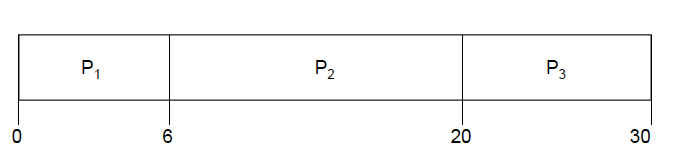
\includegraphics[width=\textwidth]{FIFO}
		\end{center}
		\begin{center}
		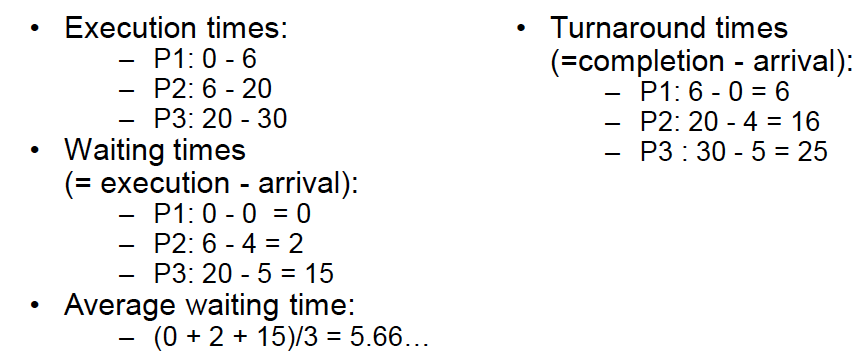
\includegraphics[width=\textwidth]{FIFOc}
		\end{center}
	\end{figure}

	\subsection{SJF}

		\par{The \ita{Shortest Job First} algorithm chooses the processes with the lowest CPU burst time to be executed first, if the processes have the same CPU burst time then it falls back to FIFO. This is also simple to implement, but an obvious problem is that processes with large CPU burst times may take much more to implement}

		\begin{figure}[H]
		\begin{center}
		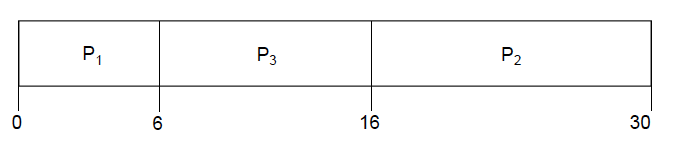
\includegraphics[width=\textwidth]{SJF}
		\end{center}
		\begin{center}
		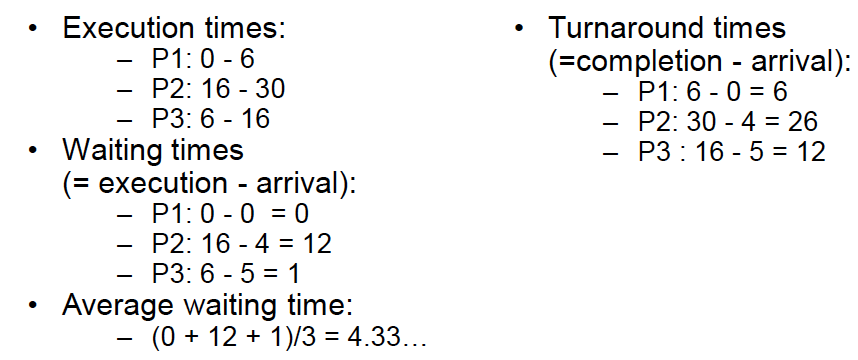
\includegraphics[width=\textwidth]{SJFc}
		\end{center}
	\end{figure}

	\subsection{SRTF}

		\par{The \ita{Shortest Remaining Time First} is a preemptive version of SJF, i.e. it looks at the list of processes in the ready queue with each new arrival and compares the total remaining completion times, if the total time of a waiting process is lower than the one currently in execution then it will interrupt execution and swap them. }

		\begin{figure}[H]
		\begin{center}
		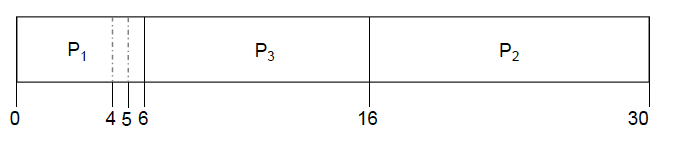
\includegraphics[width=\textwidth]{SRTF}
		\end{center}
		\begin{center}
		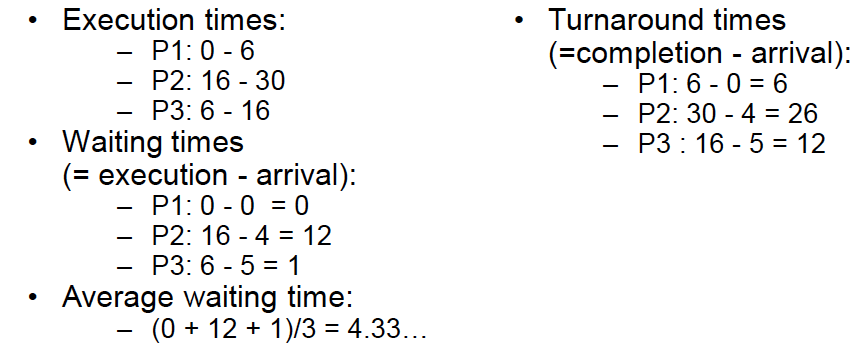
\includegraphics[width=\textwidth]{SRTFc}
		\end{center}
	\end{figure}

	\subsection{NPP}

		\par{The \ita{Non-Preemptive Priority Scheduling} adds processes to a queue according to their priority values; if processes share the same priority level, then it reverts back to FIFO. It is also fairly simple to implement, but similarly to SJF it might lead to \ita{starvation}, i.e processes with low priority may take ages or never run}

		\begin{figure}[H]
		\begin{center}
		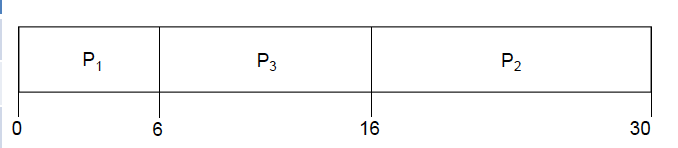
\includegraphics[width=\textwidth]{NPP}
		\end{center}
		\begin{center}
		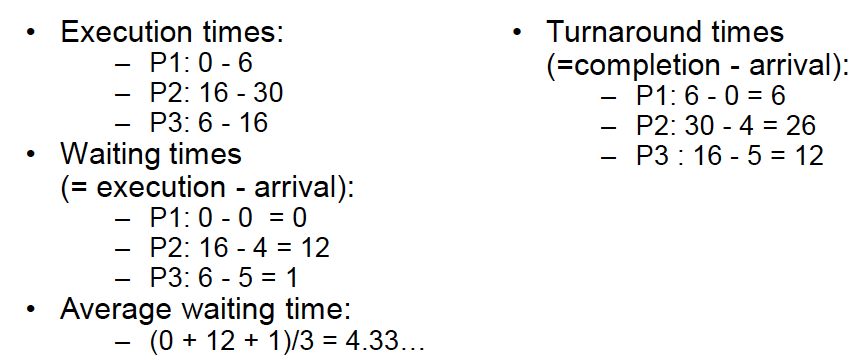
\includegraphics[width=\textwidth]{NPPc}
		\end{center}
	\end{figure}

	\subsection{RR}

		\par{The \ita{Round-Robin Scheduling} is the preemptive version of FIFO, where processes are executed according to time of arrival but only for a certain time period - \ita{quantum}. If the process finished early then the dispatcher moves down the queue, if the opposite happens the process is added to the back of the queue.}

		\begin{figure}[H]
		\begin{center}
		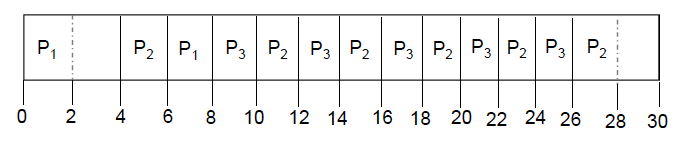
\includegraphics[width=\textwidth]{RR}
		\end{center}
		\begin{center}
		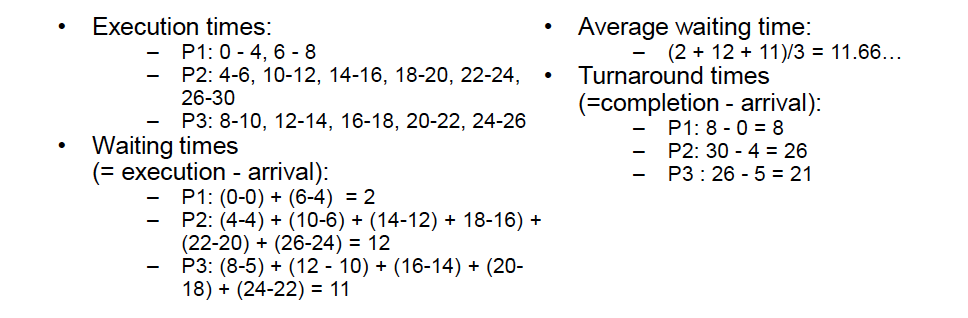
\includegraphics[width=\textwidth]{RRc}
		\end{center}
	\end{figure}

	\subsection{MQ}

		\par{The \ita{Multilevel Queue Scheduling} separates processes according to their priority values into separate queues. This has the advantage of reducing the time taken to search through all processes since it needs only to look at the highest-priority queue. It is then often combined with RR to decide which process within a queue should be executed next }




























%%%%%%%%%%%%% BIB %%%%%%%%%%%%%%%%%%%%%%%

\newpage
\nocite{*}
\printbibliography

\todos

\end{document}
